\documentclass[../main.tex]{subfiles}
\begin{document}

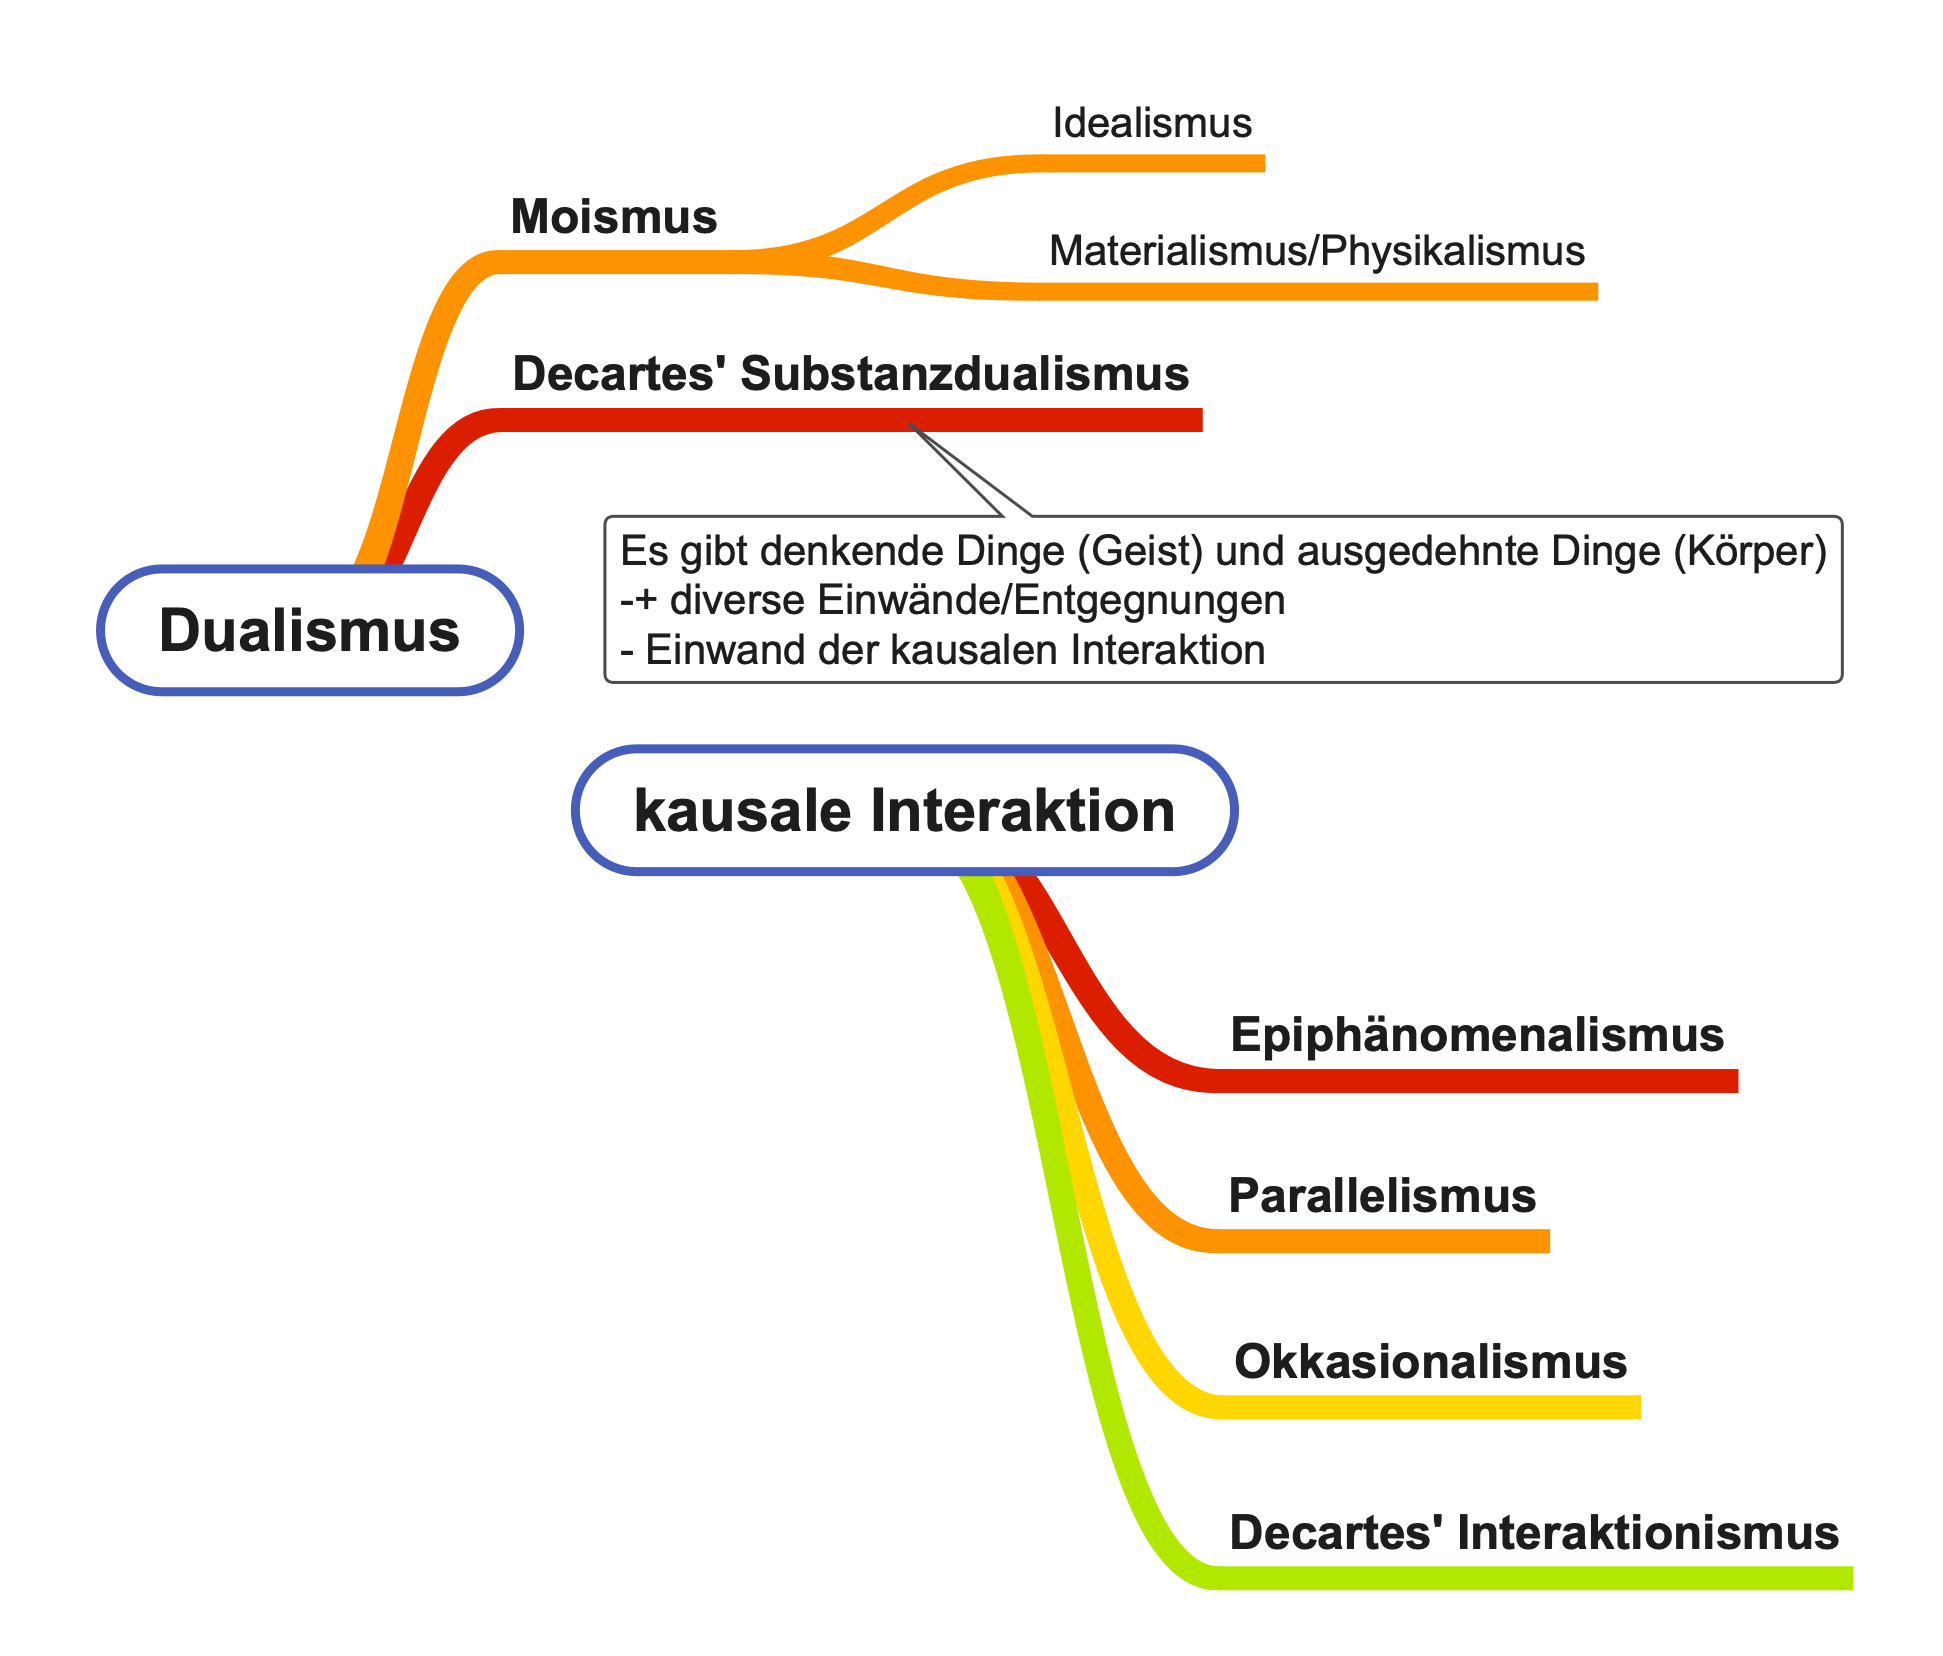
\includegraphics[width=\textwidth]{images/Dualismus_Uebersicht.png}

\section{Das Körper-Geist-Problem} 
Die Frage, inwiefern sich der Körper zum Geist/Seele und umgekehrt verhält, resp. wie sich mentale Zustände und Eigenschaften zu ihren physischen Zustände und Eigenschaften verhalten, bringt uns direkt zum Körper-Geist-Problem. 

Dieses wird aufgeteilt, in 
\begin{itemize}
	\item das \textit{Problem der mentalen Substanzen>}, das nach der Existenz von nicht-physischen, immateriellen Entitäten fragt, die Träger von mentalen Eigenschaften sein sollen und
	\item das \textit{Problem mentaler Eigenschaften}, welches die mentalen Eigenschaften auf ihre Eigenständigkeit oder ihren Ursprung in physischen Eigenschaften durchleuchtet. 
\end{itemize}

\section{Dualismus: Platon über die Seele}
\begin{enumerate}
	\item Jeder Mensch hat neben Körper auch eine Seele.
	\item Die Seele \textit{ist} der Mensch, das eigentliche Selbst. 
	\item Die Seele und der Körper sind sich unterscheidende Substanzen, die jeweils eigenständig existieren können. 
	\item Die Seele ist grundverschieden vom Körper.
\end{enumerate}

\section{Dualismus II: Descartes' Theorie von Körper und Geist (Substanzdualismus)}
\paragraph{These} 
\begin{enumerate}
	\item Es gibt zwei Arten von Substanzen/Dingen: 
	\begin{enumerate}
		\item denkende Dinge (Seelen/reine Geister)
		\item ausgedehnte Dinge (Körper)
	\end{enumerate}
	\item Die Annahme einer Seele/eines Geistes erklärt Denken (und Handeln). Alle anderen Vorgänge können durch körperliche Prozesse erklärt werden. 
\end{enumerate}
\paragraph{Argumente}
\begin{enumerate}
	\item Descartes argumentiert, dass (1) man daran zweifeln kann, ob der Körper existiert (siehe skeptische Szenarien), (2) man aber nicht daran zweifeln kann, dass man selber, also der eigene Geist, existiert, da man ja darüber nachdenken kann. Demzufolge (3) ist der Geist verschieden vom Körper. 
		
		Dieses Argument wird jedoch als ungültig erklärt, siehe Einwand Nr. 1.
	\item \textbf{Trennbarkeits-Argument} von Descartes: (1) Was erfassbar (d.h. denkbar) ist, muss metaphysisch möglich sein. (2) Da der Geist ohne einen Körper oder umgekehrt der Körper ohne Geist denkbar ist, (3) muss es metaphysisch möglich sein, dass diese zwei Dinge unabhängig voneinander existieren können. (4) Demzufolge sind Geist und Körper real verschieden, also numerische verschiedene Substanzen. 
		
		Für das Argument gibt es mögliche Einwände, siehe Einwände Nr. 2. 
	\item Descartes: Menschen haben im Vergleich zu Tieren die Fähigkeit zu sprechen und intelligent zu handeln. Aus dem folgt, dass die Tiere eine grundsätzlich andere Seele als Menschen haben. Laut Descartes haben Tiere sogar überhaupt keine Seele, sondern nur ein \textit{materielles Hirn} (verhaltenssteuerndes Organ) und der Mensch hat einen \textit{nicht-materiellen Geist}, welcher für die aufgeführten Fähigkeiten verantwortlich ist. 
		
		Für das Argument gibt es einen Haufen an Einwänden, siehe Einwände Nr. 3. 
\end{enumerate}
\paragraph{Einwände}
\begin{enumerate}
	\item Ravenscroft: Dem ersten Argument von Descartes ist folgendes, strukturanaloges Argument entgegenzusetzen, welches das Ursprungsargument \textit{ungültig} macht: Wenn (1) ich bezweifle, dass eine Person wirklich existiert ohne zu bezweifeln, dass (2) der Schöpfer einer Sache (die Person, deren Existenz wir bezweifeln) existiert, kommen wir zum Ergebnis, dass (3) der Schöpfer offensichtlich nicht die gleiche Person ist, wie die, deren Existenz wir bezweifeln. Man spricht hier von \textit{intensionaler Fehlschluss}, denn diese beiden Personen sind in Wahrheit ein und dieselbe, jedoch anders referenziert. 
	\item Zu Trennbarkeits-Argument von Descartes: Die Prämisse 1. des Argumentes lässt sich bestreiten; Nicht alles, dass man klar und deutlich erfassen (d.h. denken) kann, ist metaphysisch möglich.
	\item Zu Trennbarkeits-Argument: Es gibt noch ein Einwand bezüglich der Substanzen, der aber in der Vorlesung als <<zu kompliziert>> markiert ist. Also lassen wir diesen. 	
	\item Zum Mensch-Tier-Argument: (1) Es ist zweifelhaft, ob Descartes Beobachtungen in der Natur zutreffen (aka sie sind Bullshit) und es ist desweiteren, ohne Kenntnisse über die Natur zu haben, absonderlich, dass unser Verhalten, wenn auch etwas komplexer als die gewisser anderer Lebewesen, nicht auch einfach ein Produkt des \textit{materiellen Hirns} sind. 
\end{enumerate}

\subsection{Eigenschaftsdualismus}
Es gibt irreduzible mentale Eigenschaften, aber keine nicht-physischen mentalen Substanzen. Mentale Eigenschaften werden von physischen Substanzen (Lebewesen oder ihre Gehirne) instanziiert.

\section{Das Problem der kausalen Interaktion}
Das Problem der kausalen Interaktion besteht aus der Frage, ob es Kausalbeziehungen zwischen geistigen und körperlichen Zuständen gibt und wenn ja, welche Arten es gibt. Dafür wurden diverse, in den unteren Kapiteln beschriebene, Arten von Theorien entwickelt. 

\subsection{Derscartes' Interaktionismus (interaktionistische Dualismus)}
\begin{warningbox}
	Zustand im Körper $\longleftrightarrow$ Zustand im Geist
\end{warningbox}

\paragraph{Erklärung}Zustände im Körper verursachen Zustände im Geist (z.B. Verletzung --> Schmerz) und umgekehrt verursachen Zustände im Geist Zustände im Körper (z.B. Wunsch --> Handlung).

Dabei ist der Ort der kausalen Interaktion zwischen dem Geist und dem Körper die Zirbeldrüse; \textit{Wahrgenommen} wird dadurch, dass die Nerven ein <<Abbild>> (im übertragenen Sinne) der Dinge auf die Zirbeldrüse projezieren, die dann vom Geist wahrgenommen wird. Umkehrt steuert der Geist (willentliche Handlung) unter minimalem Kraftaufwand die Drehung der Zirbeldrüse so, dass <<Lebensgeister>> in die Nervenenden der für die Handlung benötigten Muskeln strömen.

\subsubsection{John Eccles Abwandlung}
John Eccles' Theorie funktioniert gleich, nur ist nicht die Zirbeldrüse ausschlaggebend, sondern ein bestimmter Teil der Hirnrinde, indem Geist und Körper direkt interagieren.

\paragraph{Probleme für Decartes und Eccles} 
\begin{enumerate}
	\item Aus welchen Gründen kann der Geist nur auf bestimmte Bereiche des Hirns einwirken?
	\item Neurobiologische Untersuchungen haben bisher keinerlei Anhaltspunkte für das Wirken nicht-physiologischer Ursachen gegeben. 
	\item Warum sollte sich der Geist nur auf die Bewegung einer bestimmten kleinen Sache beschränken? Reicht seine Kraft nicht weiter (Telekinese)?
	\item Wenn der Körper und das Gehirn nur da sind, um <<Befehle>> des Geistes auszuführen und Bericht zu erstatten (Sinneseindrücke), warum benötigt es ein derart grosses Gehirn, wenn doch das Gros der Arbeit im immateriellen Geist geschieht?

		Das Gehirn scheint also einige Aufgaben zu übernehmen. Zum Beispiel ist Teil der Verarbeitung von Sinneseindrücken die Einordnung in die umgebende Welt (Konstruktion dieser mit Sinneseindrücken). Ebenfalls sind Teile bei der Handlungsplanung involviert. \textbf{Was bleibt dem Geiste übrig?}
	\item Wie kommt es, dass mein Gehirn auf mein Körper einwirken kann, aber auf keinen anderen? Eine räumliche Relation ist auszuschliessen, da der Geist ja immateriell ist. Besteht vielleicht eine Art <<Affinitiät>> zwischen Geist und Körper? Oder ist es einfach eine weitere unerklärliche Tatsache?
	
\end{enumerate}
\paragraph{Einwände für Decartes (und Eccles)}
\begin{enumerate}
	\item Elisabeth von der Pfalz von Böhmen, 1643: Kausale Einwirkung (von Geist auf Körper und umgekehrt) erfordert einen Berührungspunkt im Raum. Wenn wir den Geist als nicht-ausgedehntes, nicht-räumliches Dinge verstehen, dann kann dieser den Körper nicht berühren. Deswegen ist die kausale Interaktion unmöglich!
\end{enumerate}

\subsection{T. H. Huxley's Epiphänomenalismus}
\begin{warningbox}
	Zustand im Körper $\longrightarrow$ Zustand im Geist
\end{warningbox}
Zustände im Geist werden zwar durch Zustände im Körper verursacht, haben aber niemals Wirkungen auf den Körper. 

\subsection{Leibniz's Parallelismus}
\begin{warningbox}
	Zustand im Körper $\xleftrightarrow{\text{prästabilierte Harmonie}}$ Zustand im Geist
\end{warningbox}
Zwar gibt es einen systematischen Zusammenhang zwischen Zuständen im Körper und Zuständen im Geist, diese beruhen aber nicht auf der Kausalbeziehung, sondern auf einer \textit{prästabilierten Harmonie}. D.h. Gott hat es so eingerichtet, dass Zustände im Körper Zuständen im Geist entsprechen.

\subsection{Malebranche's Okkasionalismus}
\begin{warningbox}
	Zustand im Körper $\xleftrightarrow{\text{göttliche Intervention}}$ Zustand im Geist
\end{warningbox}
Zwar gibt es einen systematischen Zusammenhang zwischen Zuständen im Körper und Zuständen im Geist, diese beruhen aber nicht auf der Kausalbeziehung oder einer prästabilierten Harmonie, sondern auf der göttlichen Intervention, die anlässlich gewisser Zustände im Einen, Zustände im Anderen auslöst. 


\section{Post-cartesischer Dualismus}
Nach Descartes war der \textit{interaktionistische Substanzdualismus} lange Zeit die dominante Position in der Philosophie des Geiste. Vertreten wurde sie durch Richard Swinburne, Alvin Plantinga, etc.

Der Dualismus wurde aber auch in Form des \textit{epiphänomenalistischen Dualismus} vertreten, der besagt, dass mentale Zustände physische Ursachen haben, aber keine physischen Wirkungen.  

\section{Monismus}
\subsection{Idealismus}
Alle physischen Entitäten lassen sich auf mentale Entitäten zurückführen.
\subsection{Materialismus/Physikalismus}
Alle Entitäten lassen sich auf physische Entitäten zurückführen.


\end{document}